%%%%%%%%%%%%%%%%%%%%%%%%%%%%%%%%%%%%%%%%%%%%%%%%%%%%%%%%%%%%%%%%%%%%%%
% LaTeX Example: Project Report
%
% Source: http://www.howtotex.com
%
% Feel free to distribute this example, but please keep the referral
% to howtotex.com
% Date: March 2011 
% 
%%%%%%%%%%%%%%%%%%%%%%%%%%%%%%%%%%%%%%%%%%%%%%%%%%%%%%%%%%%%%%%%%%%%%%
% How to use writeLaTeX: 
%
% You edit the source code here on the left, and the preview on the
% right shows you the result within a few seconds.
%
% Bookmark this page and share the URL with your co-authors. They can
% edit at the same time!
%
% You can upload figures, bibliographies, custom classes and
% styles using the files menu.
%
% If you're new to LaTeX, the wikibook is a great place to start:
% http://en.wikibooks.org/wiki/LaTeX
%
%%%%%%%%%%%%%%%%%%%%%%%%%%%%%%%%%%%%%%%%%%%%%%%%%%%%%%%%%%%%%%%%%%%%%%
% Edit the title below to update the display in My Documents
%\title{Project Report}
%
%%% Preamble
\documentclass[paper=a4, fontsize=11pt]{scrartcl}
\usepackage[T1]{fontenc}
\usepackage{fourier}

\usepackage[english]{babel}															% English language/hyphenation
\usepackage[protrusion=true,expansion=true]{microtype}	
\usepackage{amsmath,amsfonts,amsthm} % Math packages
\usepackage[pdftex]{graphicx}	
\usepackage{url}
\usepackage{subcaption}
%%% Custom sectioning
\usepackage{sectsty}
\allsectionsfont{\centering \normalfont\scshape}


%%% Custom headers/footers (fancyhdr package)
\usepackage{fancyhdr}
\pagestyle{fancyplain}
\fancyhead{}											% No page header
\fancyfoot[L]{}											% Empty 
\fancyfoot[C]{}											% Empty
\fancyfoot[R]{\thepage}									% Pagenumbering
\renewcommand{\headrulewidth}{0pt}			% Remove header underlines
\renewcommand{\footrulewidth}{0pt}				% Remove footer underlines
\setlength{\headheight}{13.6pt}


%%% Equation and float numbering
\numberwithin{equation}{section}		% Equationnumbering: section.eq#
\numberwithin{figure}{section}			% Figurenumbering: section.fig#
\numberwithin{table}{section}				% Tablenumbering: section.tab#


%%% Maketitle metadata
\newcommand{\horrule}[1]{\rule{\linewidth}{#1}} 	% Horizontal rule

\title{
		%\vspace{-1in} 	
		\usefont{OT1}{bch}{b}{n}
		\normalfont \normalsize \textsc{Udacity Autonomous Driving Car} \\ [25pt]
		\horrule{0.5pt} \\[0.4cm]
		\huge Project 2 Traffic sign classifier \\
		\horrule{2pt} \\[0.5cm]
}
\author{
		\normalfont 								\normalsize
        \today
}
\date{}


%%% Begin document
\begin{document}
\maketitle
\section{rubic point}
Project 2 and corresponding course talked about use Tensorflow to implement traffic signs classification use LeNet architecture. 

\begin{enumerate}
\item Provide a basic summary of the data set.

The size of training set is $39200 \times 32 \times 32 \times 3$, the validation size is  $39200 \times 32 \times 32 \times 3$ and the test size is $39200 \times 32 \times 32 \times 3$. The shape of each traffic sign image is $39200 \times 32 \times 32 \times 3$. The unique classes in the data set is $43$. The training images with each class are illustrated in Fig \ref{fig:originalimage}
\begin{figure}
  \centering
  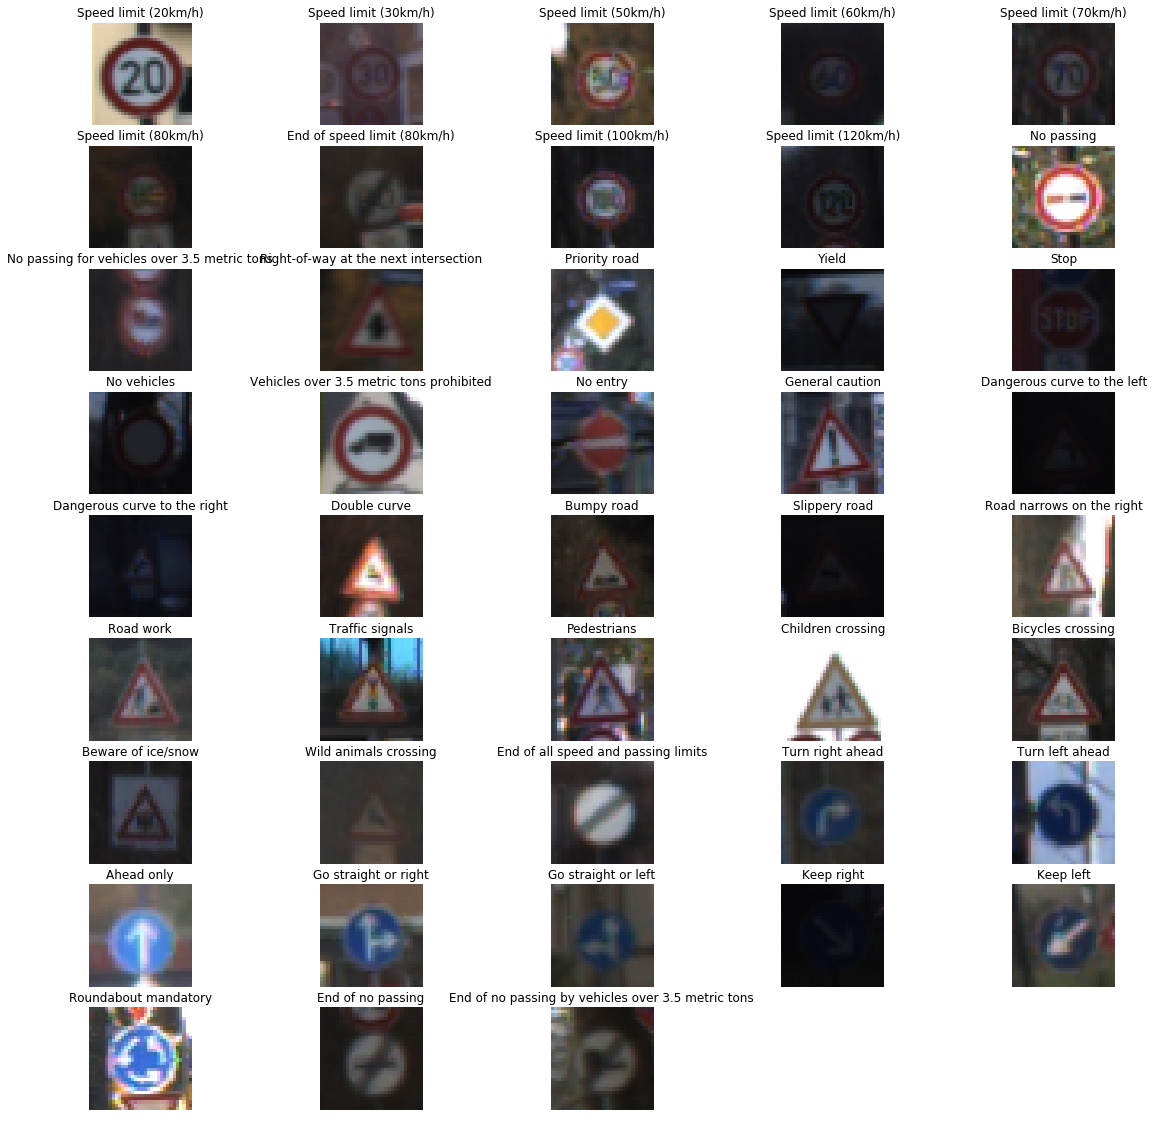
\includegraphics[width=1.0\linewidth]{trainimg.png}
  \caption{Illustration of the original training images.}
  \label{fig:originalimage}
\end{figure} 

\item Include an exploratory visualization of the dataset. 
\begin{figure}
  \centering
  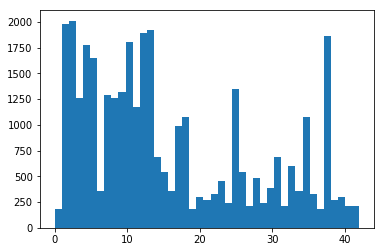
\includegraphics[width=.8\linewidth]{datahist.png}
  \caption{Histogram figure of training data}
  \label{fig:datahist}
\end{figure}
From Fig \ref{fig:datahist}, we can tell the distribution of each class is not equal. This may bring the problem of bias for the network work.

\item Describe how you preprocessed the image data. What techniques were chosen and why did you choose these techniques?

Generally speaking, I mainly consider normalize or scale the image data. More specifically, I used two different normalization methods, min-max scaling and zero-score scaling. I think the color information is useful, therefore, the grayscale is not employed in my implementation. I tried directly using the original image, using min-max scaling and zero-score scaling. The results can be significant different. Directly using original training data achieved less than $80\%$ training accuracy. However, using zero-score I achieved $99\%$ training accuracy and $93\%$ testing accuracy. The improvement is significant.
\begin{figure}
  \centering
  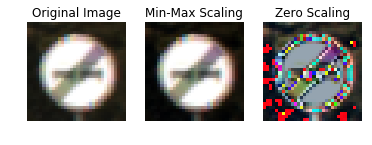
\includegraphics[width=.8\linewidth]{normalization.png}
  \caption{Normalize the training image}
  \label{fig:normalization}
\end{figure} 

\item Describe what your final model architecture looks like including model type, layers, layer sizes, connectivity, etc.

My final model is almost exactly the same with classic LeNet-5 layers. More specifically, I have the following layers:


\begin{center}
\begin{tabular}{ c c }
 Layer & Description\\ 
 Input & $32 \times 32 \times 3$\\  
 Convolution $3 \times 3$& 1x1 stride, same padding, filter size: $5 \times 5 \times 3 \times 6$\\
 Activation layer & ReLu layer \\
 Pooling Layer & Max pooling layer 2x2 stride \\
 Dropout Layer & Prob = 0.5 \\
 
  Input & $32 \times 32 \times 3$\\  
 Convolution $3 \times 3$& x1 stride, same padding, filter size: $5 \times 5 \times 6 \times 16$\\
 Activation layer & ReLu layer \\
 Pooling Layer & Max pooling layer 2x2 stride \\
 Dropout Layer & Prob = 0.5 \\
 
Fully connected (dense) layer & input size 400, output size 120\\
Fully connected (dense) layer & input size 120, output size 84\\
Fully connected (dense) layer & input size 84, output size 43\\
 
\end{tabular}
\end{center}

\item Describe how you trained your model. The discussion can include the type of optimizer, the batch size, number of epochs and any hyperparameters such as learning rate.

To train the model, I used an Adam optimizer, and set epoch size as 20, batch size as 128, the initial learning rate as 0.001.

\item Describe the approach taken for finding a solution and getting the validation set accuracy to be at least 0.93. 

My final model results with each epoch are:
EPOCH 1: Training Accuracy = 0.742, Validation Accuracy = 0.702 \\
EPOCH 2: Training Accuracy = 0.879, Validation Accuracy = 0.831 \\
EPOCH 3: Training Accuracy = 0.922, Validation Accuracy = 0.876 \\
EPOCH 4: Training Accuracy = 0.948, Validation Accuracy = 0.902 \\
EPOCH 5: Training Accuracy = 0.959, Validation Accuracy = 0.923 \\
EPOCH 6: Training Accuracy = 0.962, Validation Accuracy = 0.912 \\
EPOCH 7: Training Accuracy = 0.975, Validation Accuracy = 0.926 \\
EPOCH 8: Training Accuracy = 0.981, Validation Accuracy = 0.929 \\
EPOCH 9: Training Accuracy = 0.986, Validation Accuracy = 0.947 \\
EPOCH 10: Training Accuracy = 0.980, Validation Accuracy = 0.932 \\
EPOCH 11: Training Accuracy = 0.990, Validation Accuracy = 0.955 \\
EPOCH 12: Training Accuracy = 0.990, Validation Accuracy = 0.950 \\
EPOCH 13: Training Accuracy = 0.992, Validation Accuracy = 0.956 \\
EPOCH 14: Training Accuracy = 0.993, Validation Accuracy = 0.956 \\
EPOCH 15: Training Accuracy = 0.992, Validation Accuracy = 0.955 \\
EPOCH 16: Training Accuracy = 0.994, Validation Accuracy = 0.957 \\
EPOCH 17: Training Accuracy = 0.994, Validation Accuracy = 0.957 \\
EPOCH 18: Training Accuracy = 0.995, Validation Accuracy = 0.957 \\
EPOCH 19: Training Accuracy = 0.995, Validation Accuracy = 0.955 \\
EPOCH 20: Training Accuracy = 0.994, Validation Accuracy = 0.956 \\

I only test one final testing accuracy, and the result accuracy is: $93.73713382632602\%$
    \begin{itemize}
      \item{What was the first architecture that was tried and why was it chosen?}
      
      I tried the regular LeNet without drouput. I choose it as the most successful architecture in digits classification.
      \item{How was the architecture adjusted and why was it adjusted? }
      
      From my experience, the most significant effect is using dropout layer. Without dropout layer, my testing accuracy is around $90\%$. In other words, the testing accuracy is improved higher than $93\%$ with appending two dropout layers. I did not change the activation function since ReLu has been proved as the most effective activation function.
      \item Which parameters were tuned? How were they adjusted and why?
      
      I tuned epoch numbers, with the increase of epoch numbers the accuracy can be improved. Another parameter is learning rate. It is important because we have to trade-off between the converge speed and training loss. The rule of thumb is $0.001$.
      \item{What are some of the important design choices and why were they chosen? For example, why might a convolution layer work well with this problem? How might a dropout layer help with creating a successful model?}
      
      In my opinion, Convolutional layer works since it has much less parameters than dense layer or regular fully layer. In this way we can overcome overfitting problem. Dropout layer help the training because it works like an ensemble filter to prevent training highly depends on some particular parameters.
    \end{itemize}
    
    \item{If a well known architecture was chosen}
     \begin{itemize}
      \item{What architecture was chosen?}
       I employed LeNet architecture, which constructed by 2 convolutional layers and 3 fully connected layers.
    \item {Why did you believe it would be relevant to the traffic sign application?}
    Traffic sign classification is very similar with digits classification. And convolutional layers are good for solve the image classification problem.
    \end{itemize}
	
	\item {Test a Model on New Images}
	\begin{itemize}
	\item {Choose five German traffic signs found on the web and provide them in the report. For each image, discuss what quality or qualities might be difficult to classify.}
	The randomly selected figures are illustrated in Fig \ref{fig:5images} and the detected results are shown in Fig \ref{fig:5imagesresults}.
\begin{figure}
  \centering
  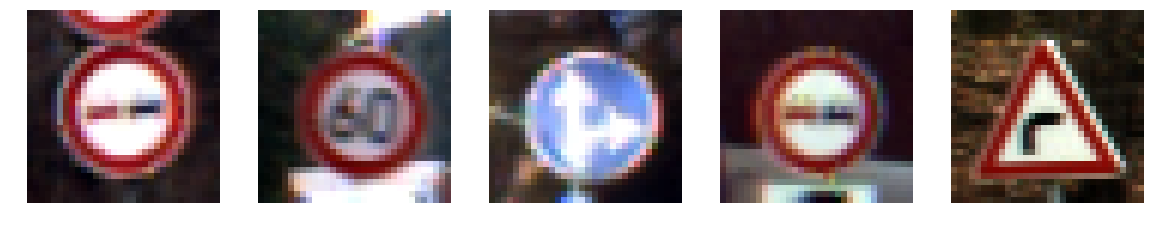
\includegraphics[width=1.0\linewidth]{5images.png}
  \caption{Illustration of 5 Germain traffic signes.}
  \label{fig:5images}
\end{figure} 
\begin{figure}
  \centering
  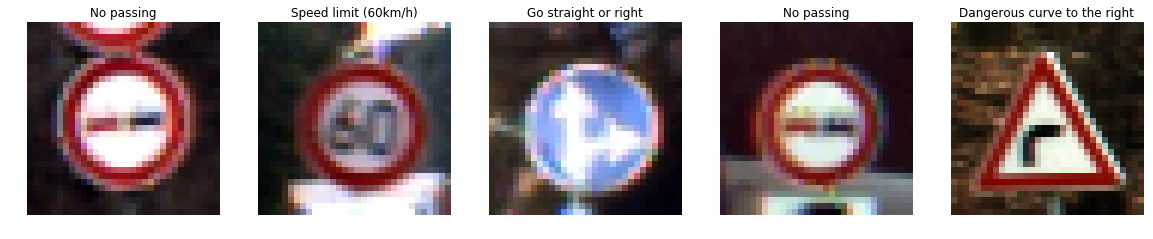
\includegraphics[width=1.0\linewidth]{5imagesresults.png}
  \caption{Illustration of 5 Germain traffic signs and detected results.}
  \label{fig:5imagesresults}
\end{figure} 
	\end{itemize}
	
	\begin{center}
\begin{tabular}{ c c }
 Image & Prediction\\ 
 No passing & No assing\\ 
 Speed limit (60km/h) & Speed limit (60km/h)\\
 Go straight or right & Go straight or right\\
 No passing & No passing \\
 Dangerous curve to the right & Dangerous curve to the right \\
\end{tabular}
\end{center}

For the first image, the model is relatively sure that this is a stop sign (probability of 0.6), and the image does contain a stop sign. The top five soft max probabilities were
\begin{center}
\begin{tabular}{ c c }
 Probability & Prediction\\ 
1 & No passing\\ 
0 & Vehicles over 3.5 metric tons prohibited\\
0 & Speed limit (50km/h)\\
0 & No passing for vehicles over 3.5 metric tons \\
0 & No vehicles\\
\end{tabular}
\end{center}

\begin{center}
\begin{tabular}{ c c }
 Probability & Prediction\\ 
0.999 & Speed limit (60km/h)\\ 
0.001 & Speed limit (80km/h)\\
0 & Speed limit (50km/h)\\
0 & Ahead only \\
0 & No passing\\
\end{tabular}
\end{center}

\begin{center}
\begin{tabular}{ c c }
 Probability & Prediction\\ 
0.837 & Go straight or right\\ 
0.154 & Keep right\\
0.009 & Turn left ahead\\
0 & End of all speed and passing limits\\
0 & End of no passing\\
\end{tabular}
\end{center}


\begin{center}
\begin{tabular}{ c c }
 Probability & Prediction\\ 
1 & No passing\\ 
0 & No passing for vehicles over 3.5 metric tons\\
0 & Speed limit (60km/h)\\
0 & Vehicles over 3.5 metric tons prohibited \\
0 & Slippery road\\
\end{tabular}
\end{center}

\begin{center}
\begin{tabular}{ c c }
 Probability & Prediction\\ 
1 & Dangerous curve to the right\\ 
0 & Children crossing\\
0 & Slippery road\\
0 & Road work\\
0 & No passing\\
\end{tabular}
\end{center}

\end{enumerate}

\section{Possible improvements}
There is no difference between deep learning and more conventional "neural network". I would like to try deeper layers (with more than 10 convolutional layers) or new architecture introduced in recent years such as ResNet to improve the classification rate.

\end{document}